\documentclass[12pt]{article}
\usepackage{amsmath}
\usepackage{fancyhdr}
\usepackage{graphicx} 
\usepackage{tikz}
\usepackage{pgfplots}
\usetikzlibrary{shapes,backgrounds}
\usepackage[margin=1in]{geometry}

\pagestyle{fancy}
\lhead{CSCI 6550}
\chead{\textbf{Week 4 Assignment Report}}
\rhead{Eric Miller}

\begin{document}
\subsection*{Methods}
For the last week, I worked primarily on extending the previous algorithms to \(N\times N\) boards. Beforehand, I worked on improving the cache for alpha-beta pruning. For every board state that is encountered, a score is stored along with a flag: 0 for exact, -1 for lower bound, and 1 for upper bound. If the score is not more than the alpha value used to get there, there may have been pruning at some point that did not allow a lower score to appear (and an upper bound flag is used). Similarly, if the score is at least as large as beta, it is treated as a lower bound. Then, when searching the cache, only those flagged as exact (0) are used. If the cached value is an upper bound, beta is updated to the upper bound if it's lower. Similarly, for a lower bound, alpha is updated to the bound if it's higher. Hence, if alpha becomes at least the value of beta, the node can immediately be pruned (either the score is at least beta or at most alpha, in which cases the node will end up being pruned).\footnote{Based on an algorithm in Chapter 2 of \textit{Memory versus Search in Games} by Dennis M. Breuker.}

For the first experiment, I tested both the cache-based DFS algorithm against the above alpha-beta (cached) algorithm, ordering moves by heuristic calculations, against higher level boards. The heuristic/evaluation method was updated to work for \(N\times N\) boards, including those with winning sequences of length \(k<N\). This was done by considering, within each line, connected subsequences of cells of length \(k\). For instance, when \(N=4\) and \(k=3\), the first and last three cells would be considered in every line of length four.

I then worked on an iterative deepening approach, where an additional cache was used to keep track of move history. This made use of three caches. The \texttt{cached\_leaf\_nodes} dictionary kept track of the leaf nodes (where nodes at \texttt{max\_depth} were considered leaves) using the alpha-beta method above. This was cleared at each iteration. The \texttt{last\_iter\_cache} stored the most recently found score for each board (even if pruned, for simplicity) and was used for move ordering. If move ordering failed to find a historical store in this cache, the evaluation/heuristic method was used (with its own cache to speed up reevaluations).

A .25 second timer was added to this method, so the algorithm would work down as many levels until time ran out. This worked up through \(9\times9\) boards, but \(10\times10\) and higher boards could not complete even one level of evaluations in time. This could be improved by creating a beam-size of, for example, 81 moves, but going up to \(9\times9\) worked for our purposes.


\subsection*{Results}
The following chart shoes the results shows a comparison of the new caching method and no caching for a move-ordering based alpha-beta pruning algorithm. For the first move, the cached version visits under a quarter of the states as the non-cached version. Also, after each agent has gone through the tree once, the score can immediately be returned, as the deterministic game (2 optimal agents) does not reach any states that were originally pruned.

\begin{center}
    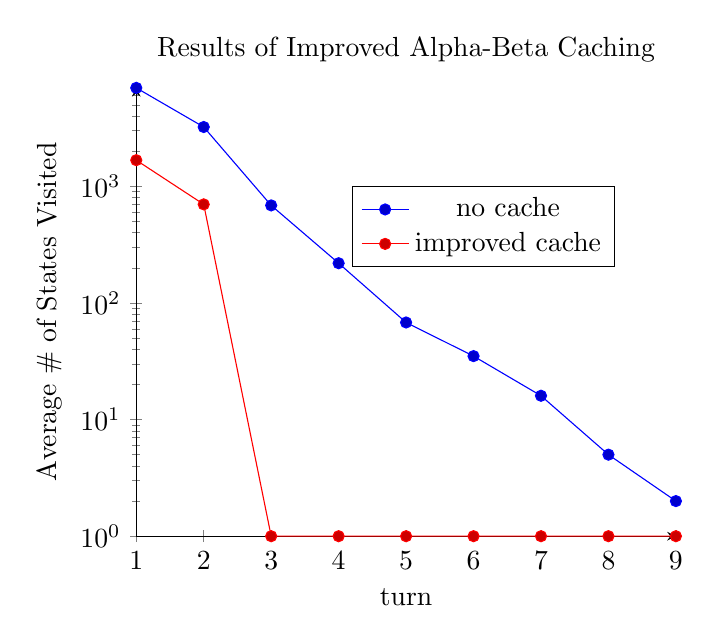
\begin{tikzpicture}
        \begin{axis}[
            legend style={at={(.4,.6)},anchor=south west},
            axis lines = left,
            xlabel = turn,
            xtick = {0, 1, 2, 3, 4, 5, 6, 7, 8, 9},
            ymode = log,
            ylabel = Average \# of States Visited,
            title = Results of Improved Alpha-Beta Caching
        ]
        \addplot+[
            mark=*,
        ] plot coordinates{
            (1,6982)
            (2,3224)
            (3,686)
            (4,219)
            (5,68)
            (6,35)
            (7,16)
            (8,5)
            (9,2)
        };
        \addlegendentry{no cache}
        \addplot+[
            mark=*,
        ] plot coordinates{
            (1,1675)
            (2,700)
            (3,1)
            (4,1)
            (5,1)
            (6,1)
            (7,1)
            (8,1)
            (9,1)
        };
        \addlegendentry{improved cache}
        
        \end{axis}
    \end{tikzpicture}
\end{center}

The following chart shows how many states are visited on the first move when we increase both \(N\) (board size) and \(k\) (winning sequence length), for both normal dfs/minimax, and an alpha-beta algorithm with move ordering. The alpha-beta agent seems to stay within a more controlled range when increasing \(N\), whereas dfs stays more controlled than alpha-beta when increasing \(k\). However, limited data is shown due to memory constraints. When \(k<N\), at least for \(k=3\) the first agent wins when playing optimally, hence decreasing the depth of the board.

\[
\begin{array}{|c|c|c|c|c|}
    \hline\mathbf{(N,k)} & (3,3) & (4,3) & (4,4) & (5,3)\\
    \hline\textbf{alpha-beta}  & 1675& 25589& 898150&696412\\
    \hline\textbf{dfs/minimax} & 16168& 23453345& 51562425&\\
    \hline
\end{array}
\]

The next graph shows a the number of states visited with iterative deepening compared to the normal algorithm (with heuristic based move ordering, same as shown in red on 2 figures up). Note that iterative deepening performs worse, as the agent must perform algorithm level-by-level, resetting each time. Iterative deepening is thus, at least for small tic-tac-toe games, not ideal if we wish to expand the entire minimax tree. Part of this is due to the fact that the heuristic works well for move ordering.

\begin{center}
    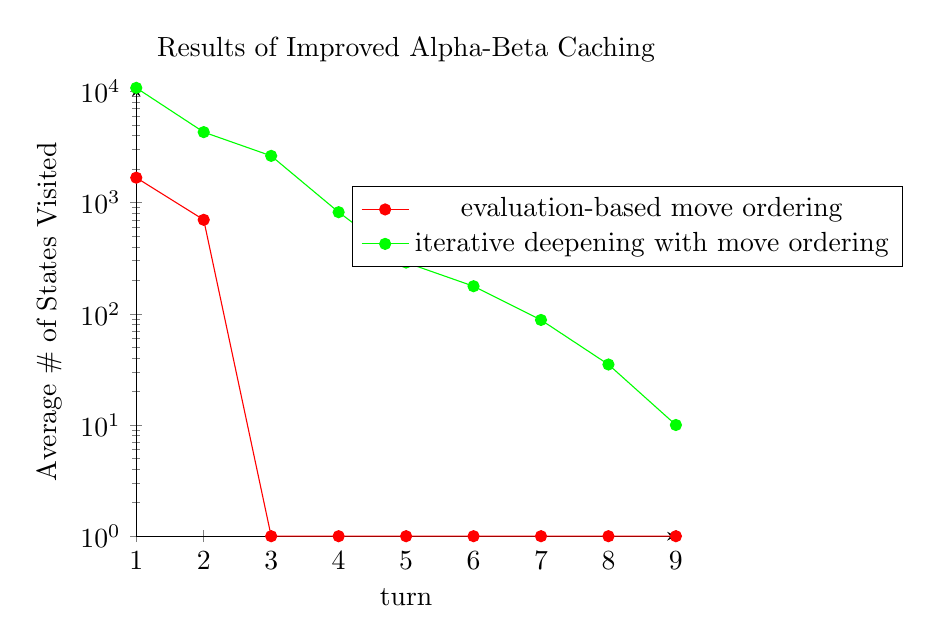
\begin{tikzpicture}
        \begin{axis}[
            legend style={at={(.4,.6)},anchor=south west},
            axis lines = left,
            xlabel = turn,
            xtick = {0, 1, 2, 3, 4, 5, 6, 7, 8, 9},
            ymode = log,
            ylabel = Average \# of States Visited,
            title = Results of Improved Alpha-Beta Caching,
        ]
        \addplot[
            mark=*,
            color=red
        ] plot coordinates{
            (1,1675)
            (2,700)
            (3,1)
            (4,1)
            (5,1)
            (6,1)
            (7,1)
            (8,1)
            (9,1)
        };
        \addlegendentry{evaluation-based move ordering}
        \addplot[
            green,
            mark=*,
        ] plot coordinates{
            (1,10755)
            (2,4302)
            (3,2631)
            (4,820)
            (5,289)
            (6,177)
            (7,88)
            (8,35)
            (9,10)
        };
        \addlegendentry{iterative deepening with move ordering}
        
        \end{axis}
    \end{tikzpicture}
\end{center}

Placing a .25 second time limit on the agent fixed this issue, while maintaining some level of optimality through heuristics. The following graph shows the number of wins of 25 games for each board size (where \(k=N\)).

\begin{center}
    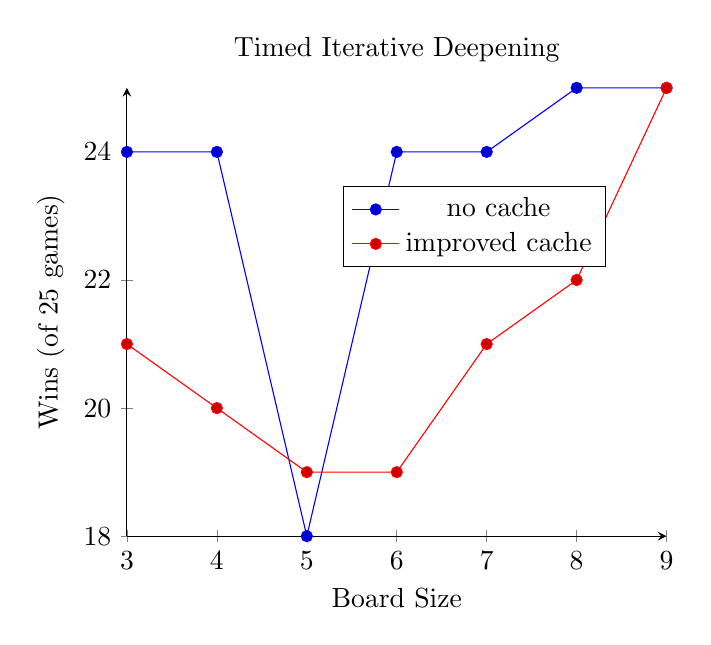
\begin{tikzpicture}
        \begin{axis}[
            legend style={at={(.4,.6)},anchor=south west},
            axis lines = left,
            xlabel = Board Size,
            xtick = {0, 1, 2, 3, 4, 5, 6, 7, 8, 9},
            ylabel = Wins (of 25 games),
            title = Timed Iterative Deepening
        ]
        \addplot+[
            mark=*,
        ] plot coordinates{
            (3,24)
            (4,24)
            (5,18)
            (6,24)
            (7,24)
            (8,25)
            (9,25)
        };
        \addlegendentry{no cache}
        \addplot+[
            mark=*,
        ] plot coordinates{
            (3,21)
            (4,20)
            (5,19)
            (6,19)
            (7,21)
            (8,22)
            (9,25)
        };
        \addlegendentry{improved cache}
        
        \end{axis}
    \end{tikzpicture}
\end{center}

In reality, the higher level games are easier to win against a random player, as there is more board space for the random agent to "miss" blocking the iterative-deepening agent. Against any agent with some understanding of strategy, it would be extremely easy to block any win, and most games would end in draws. However, especially at the lower level boards, the proportion of wins seems to show that the agent can play somewhat optimally, even without fully expanding the minimax tree. It is also notable that the random algorithm never won, even when going first.

\end{document}